\documentclass{paper}

\usepackage{authblk}
\usepackage{hyperref}
\usepackage{graphicx}

\bibliographystyle{ieeetr}

\graphicspath{ {../assets/} } 

\author[1]{Alexandre Silva, \emph{alexandre.silva1@unesp.br}}
\affil[1]{Ibilce - Instituto de Biociências, Letras e Ciências Exatas - Câmpus de São José do Rio Preto - Unesp}

\title{Atividade 1 - Modelos de Classificação}

\begin{document}

\maketitle

\section{Introdução}

Durante as aulas de mineração de dados, nos foi dada a seguinte tarefa,

\begin{verbatim}
Selecionar 1 conjunto de dados que contenha ao menos 4 classes. 
Utilize o pré-processamento que julgar adequado. 
Aplicar sobre o conjunto os seguintes algoritmos: árvore, bagging, 
boosting (pode ser o AdaBoost), Random Forest. Avaliar quais deles 
gera o melhor modelo usando para tanto alguma técnica de validação (holdout, etc.).
Escolha uma medida para avaliar o desempenho (acurácia, F1, etc.). 
Considerando o de melhor resultado, faça a setagem de hiperparâmetros 
no mesmo para ver se o desempenho melhora.

Transformar o problema multiclasse em problemas binários usando OVA e OVO. 
Escolha uma medida para avaliar o desempenho (acurácia, F1, etc.) e diga 
qual das duas abordagens se saiu melhor usando para tanto alguma 
técnica de validação (holdout, etc.). Use como algoritmo o de árvore.
\end{verbatim}

Aqui, mostrarei minha solução para esta atividade, detalhando cada aspecto e aprendizado retido durante o desenvolvimento.

Para realizar este trabalho, foram utilizados as seguintes ferramentas: \textbf{Python3}, \textbf{pandas}, \textbf{matplotlib}, \textbf{seaborn}, \textbf{uv}, \textbf{kagglehub}, \textbf{JupyterLab}, \textbf{make}, \textbf{scikit-learn} e \textbf{numpy}. Para mais informações, é referenciado aqui o repositório do Github contendo todos os notebooks com os testes e desenvolvimento dos modelos \url{https://github.com/Dpbm/mestrado-aulas/tree/main/mineracao-de-dados/atividades/atividade1}.

\section{Dataset}

O dataset escolhido tem o título \textbf{Machine Predictive Maintenance Classification}, e encontra-se no \textit{Kaggle} através do link: \url{https://www.kaggle.com/datasets/shivamb/machine-predictive-maintenance-classification}.

Neste  \textit{dataset}, são dados informações sobre máquinas e suas condições de operação. Tal conjunto de dados, apresenta duas colunas objetivo. A primeira (de nome \textit{`Target`}), tem a finalidade da prever a falha de uma máquina de forma binária, ou seja, se ela vai ou não falhar. Por outro lado a segunda (de nome \textit{`Failure Type`}), categoriza os tipos de falha. Esta pode conter os seguintes valores: \texttt{['No Failure', 'Power Failure', 'Tool Wear Failure', 'Overstrain Failure', 'Random Failures', 'Heat Dissipation Failure']}.

No total, o conjunto compreende $10000$ linhas com $6$ colunas, não possuindo dados faltantes ou valores nulos a serem tratados.

Segue a descrição completa do \textit{dataset},

\begin{verbatim}

Since real predictive maintenance datasets are generally difficult to 
obtain and in particular difficult to publish, we present and provide a 
synthetic dataset that reflects real predictive maintenance encountered in 
the industry to the best of our knowledge.

The dataset consists of 10 000 data points stored as rows with 14 features in columns

UID: unique identifier ranging from 1 to 10000
productID: consisting of a letter L, M, or H for low (50% of all products), 
medium (30%), and high (20%) as product quality variants and a 
variant-specific serial number
air temperature [K]: generated using a random walk process later 
normalized to a standard deviation of 2 K around 300 K
process temperature [K]: generated using a random walk process 
normalized to a standard deviation of 1 K, added to the air temperature plus 10 K.
rotational speed [rpm]: calculated from powepower of 2860 W, overlaid 
with a normally distributed noise
torque [Nm]: torque values are normally distributed around 40 Nm 
with an σ = 10 Nm and no negative values.
tool wear [min]: The quality variants H/M/L add 5/3/2 minutes of tool
wear to the used tool in the process. and a
'machine failure' label that indicates, whether the machine has failed in 
this particular data point for any of the following failure modes are true.
Important : There are two Targets - Do not make the mistake of using 
one of them as feature, as it will lead to leakage.
Target : Failure or Not
Failure Type : Type of Failure

\end{verbatim}


\section{Análises}

O primeiro passo para este trabalho, foi a exploração inicial dos dados. Nosso objetivo aqui é entender como os dados estão estruturados, suas correlações. Possíveis \textit{features} e demais informações relevantes para a criação de um modelo.

\subsection{Distribuição de classes}

A primeira análise feita, foi em relação à como os dados estavam distribuídos por classes.

\begin{figure} \label{fig:targets}
	\centering
	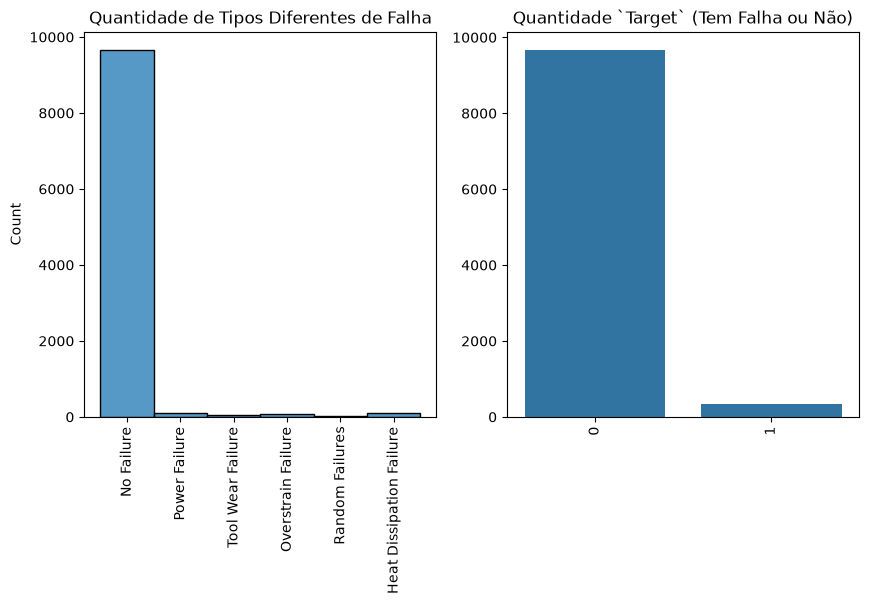
\includegraphics[width=\linewidth]{quantidade-por-label-targets}
	\caption{Distribuição de valores por classe.}
\end{figure}

Como mostrado na Figura~\ref{fig:targets}, as classes não possuíam balanceamento adequado, sendo a classe majoritária a classe referente a máquinas sem falha. Este é um fator preocupante ao treinar um modelo, dado que dados neste formato poderiam levar a \textit{overfitting}, incentivando o modelo a sempre `chutar` na classe majoritária. Para resolver esta questão, posteriormente foi realizado o processo de \textit{Data Augmentation}, do qual será descrito na Seção~\ref{sec:aug}.

Com isso, foram repartidos os dados em dois \textit{dataframes} distintos. O primeiro contendo os valores que possuíam e o outro os que não apresentavam falha, filtro aplicado com base na coluna \textit{Target} por valores $1$ e $0$ respectivamente.

Ainda com relação a distribuição das classes, notou-se que algumas falhas estavam classificadas de forma errada perante a coluna \textit{Target}, como pode ser visto na Figura~\ref{fig:errado}.

\begin{figure} \label{fig:errado}
	\centering
	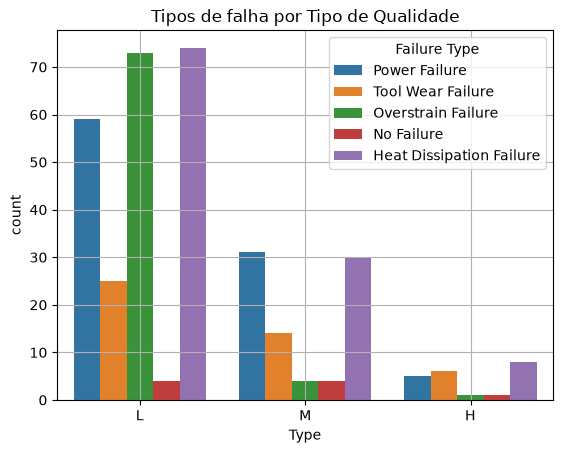
\includegraphics[width=0.8\linewidth]{tipos-de-falha-por-qualidade}
	\caption{Gráfico de tipos de Falha por qualidade da máquina. Nota-se o aparecimento da classe \textit{No Failure} na divisão que deveria conter apenas linhas com falha.}
\end{figure}

Assim, foi feita uma limpeza nos dados nas duas divisões, mantendo apenas aqueles que se enquadravam em sua designada divisão.

De forma análoga, notou-se que valores com classificada \textit{Random Failures}, estavam concentrados apenas na divisão referente à máquinas sem falha. Dessa forma, esta classificação foi totalmente removida dos dados finais.

\subsection{Quantidade de itens por Qualidade}

Dado a descrição do \textit{dataset}, sabia-se que cada item possuía uma letra associada para cada tipo de qualidade de produto sendo eles: \textit{L (Low Quality)}, \textit{M (Medium Quality)} e \textit{H (High Quality)}. 

Na própria descrição, era mostrado a proporção de dados por qualidade, contudo era necessário entender como estes estavam dentre os conjuntos separados que foram criados, o qual pode ser visto na Figura~\ref{fig:qualy-splits}.

\begin{figure}[h] \label{fig:qualy-splits}
	\centering
	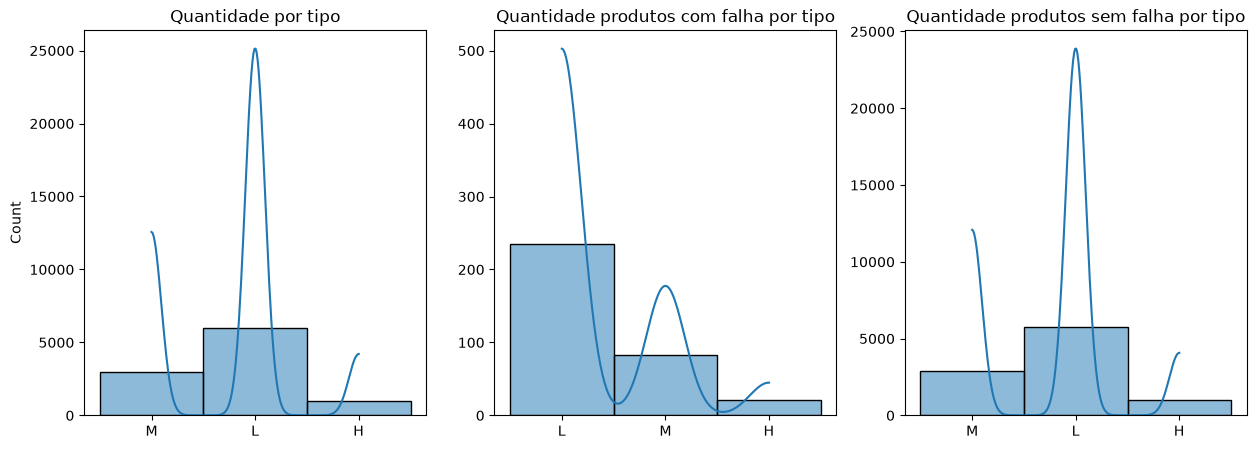
\includegraphics[width=\linewidth]{quantidade-por-tipo-qualidade}
	\caption{Quantidade de itens por qualidade e por divisão dos dados.}
\end{figure}

Notavelmente máquinas de menor qualidade são as predominantes, mas isto não se mostrou um problema mais a frente no projeto.

De forma mais minuciosa, foi verificado a quantidade de defeitos por classe, assim como feito anteriormente na Figura~\ref{fig:errado}, com os dados limpos na Figura~\ref{fig:dist-limpo}.

\newpage

\begin{figure}[h] \label{fig:dist-limpo}
	\centering
	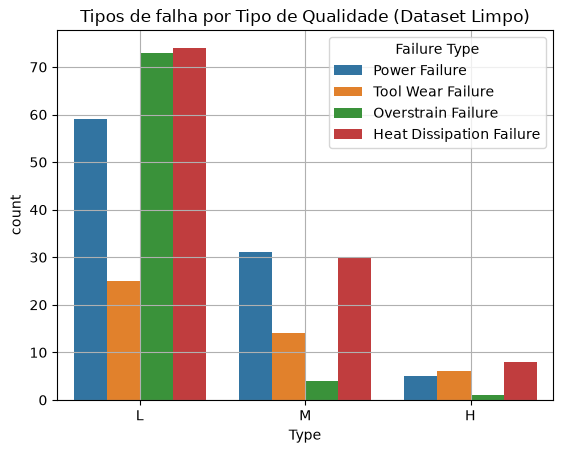
\includegraphics[width=0.8\linewidth]{tipos-de-falha-por-qualidade-limpo}
	\caption{Gráfico de tipos de Falha por qualidade da máquina. Mesmo da Figura~\ref{fig:errado}, mas dessa vez com os dados limpos.}
\end{figure}

A principio, nota-se uma certa discrepância entre as quantidades de forma geral. Assim, posteriormente empregamos o já citado \textit{Data Augmentation} para dar mais exemplos para o modelo (veja a Seção~\ref{sec:aug}).


\subsection{Entendimento do domínio}

Após a limpeza dos dados e o breve reconhecimento de suas distribuições, uma rápida pesquisa na internet foi feita para entender o que causa cada tipo de problema \cite{Power,Wear,Overstrain,Temp}.

Com base nas pesquisas, chegou-se as seguintes definições:

\begin{itemize}
	\item \textbf{Power Failure}: Quando há a perda de energia repentinamente. Fazendo com que máquinas parem de forma abrupta, e ao retornar ao trabalho podem receber picos indevidos de energia, frequência da rede instável e oscilações que podem prejudicar o equipamento;
	\item \textbf{Tool Wear Failure}: Resultado de contato/atrito que desgasta o equipamento e pode levar a falhas;
	\item \textbf{Overstrain}: quando a relação Torque (Nm) x Minutos de operação (Min)  excedem: $11{,}000$ para equipamentos \textit{L}, $12{,}000$ para \textit{M} e $13{,}000$ para \textit{H};
	\item \textbf{Heat Dissipation Failure}: Quando há calor excessivo sendo gerado em um equipamento.
\end{itemize}

\subsubsection{Overstrain}

De antemão, \textit{Overstrain} se mostrou o mais simples dos métodos para classificar. Como o problema é tido como a multiplicação entre Torque e Minutos de operação, foi feita uma breve manipulação dos dados criando assim esta nova \textit{feature} denominada \textit{Nm $\times$ Min}.

\begin{figure}[h] \label{fig:overstrain}
	\centering
	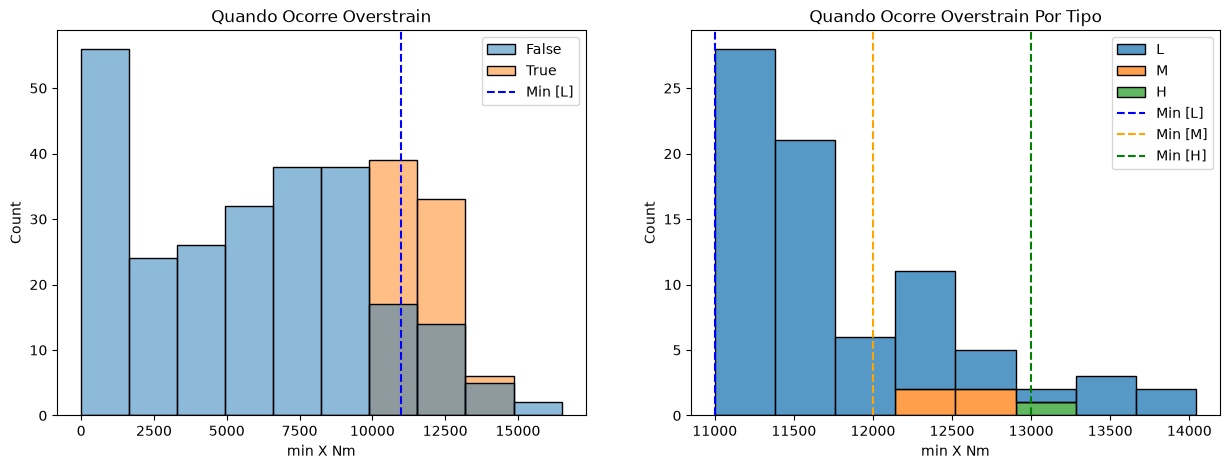
\includegraphics[width=\linewidth]{pontos-de-corte-overstrain}
	\caption{Pontos de corte para falhas por \textit{Overstrain (exaustão/sobrecarga)}.}
\end{figure}

Com uma rápida análise, é notável os pontos de corte no Gráfico~\ref{fig:overstrain}, os quais seguem exatamente o descrito.

Esta informação apresentou indícios de que apresentar ao modelo esta nova \textit{feature} ao invés dos dados separados poderia trazer benefícios.


\subsubsection{Falha por Dissipação de Calor (Heat Dissipation Failure)}

Em seguida, foram testados variáveis que poderiam estar relacionadas a geração de calor.

\begin{figure}[h] \label{fig:heat-vars-dist}
	\centering
	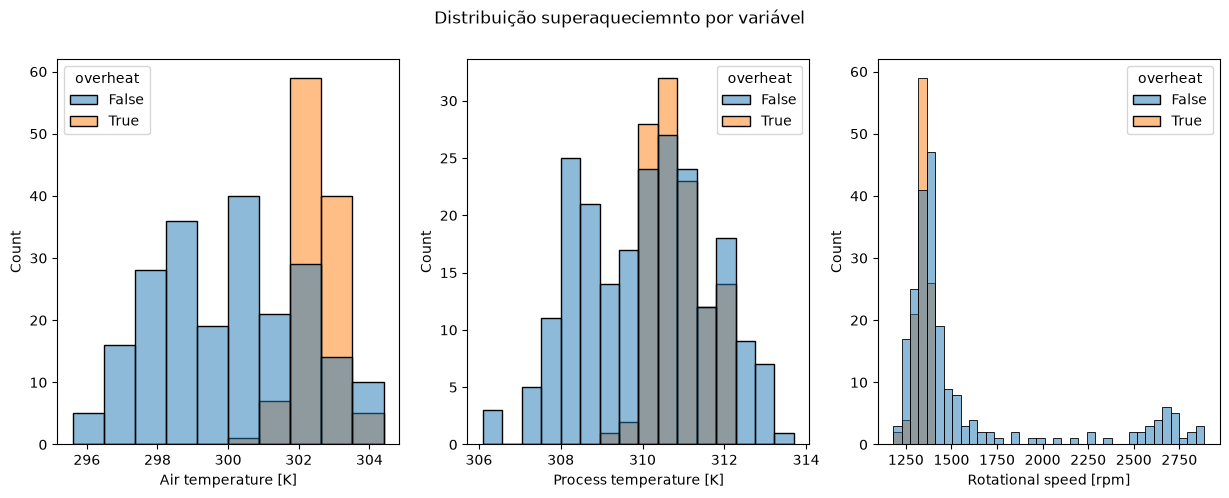
\includegraphics[width=\linewidth]{dist-overheat-temp-rpm}
	\caption{Relação de distribuição de possíveis variáveis associadas à falhas por dissipação de calor.}
\end{figure}

As primeiras colunas utilizadas para o estudo, foram as temperaturas do ar e de processo, assim como a rotação em RPM. O que foi evidenciado aqui, são alguns padrões em relação à temperatura do ar e a rotação. Neste caso, foi visto que temperaturas do ar acima de $300$ e rotações em torno de $1250$ são os que mais apresentam falha por superaquecimento.

Posteriormente, durante testes para falhas por \textit{tool wear}, foi feito um estudo mais aprofundado na distribuição de rotação por torque, como mostra a Figura~\ref{fig:torque-rpm}. A relação que se chegou é que a maior parte das máquinas estão na faixa dos $\approx 1250 RPM$, além disso maquinas de maior rotação tem menor torque, enquanto menor rotação possuem maior torque. 

Com essa informação pode-se julgar possível a hipótese de que: \textbf{máquinas de menor rotação (então possuem maior torque), são designadas para maior peso em seus eixos, contudo isso pode levar à superaquecimento conforme o esforço feito.}

Dada esta hipótese, testou-se o uso de um artificio semelhante ao Torque por minutos de trabalho, desta vez Torque por Rotação.

\newpage

\begin{figure}[h] \label{fig:torque-por-rotação}
	\centering
	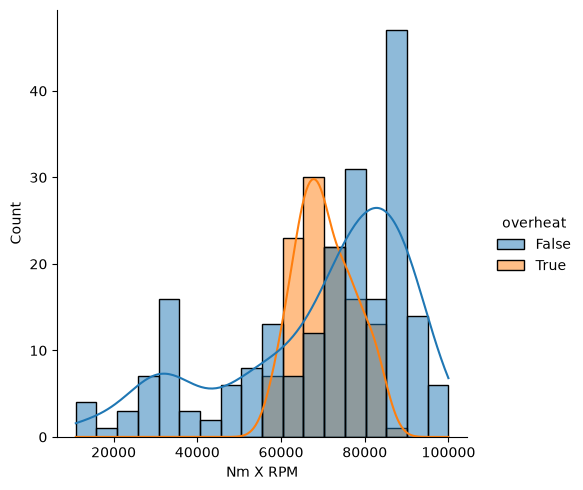
\includegraphics[width=0.8\linewidth]{overheat-torque-por-rpm}
	\caption{Problemas de \textit{overheat} relacionado à Torque por Rotação.}
\end{figure}

Neste caso, Figura~\ref{fig:torque-por-rotação}, notou-se um claro intervalo centrado entre $60000$ e $80000 Nm \times RPM$. 

De certa forma, acreditava-se que apenas esta relação poderia ser usada. Contudo, ao correlacionar ambos pontos, vimos um certo padrão, Figura~\ref{fig:ar-rpm}. Usando os dois dados, um \textit{cluster} bem definido se forma em uma região do espaço, assim temperatura do ar se mostraram como possíveis \textit{features} a serem escolhidas.


\begin{figure}[h] \label{fig:ar-rpm}
	\centering
	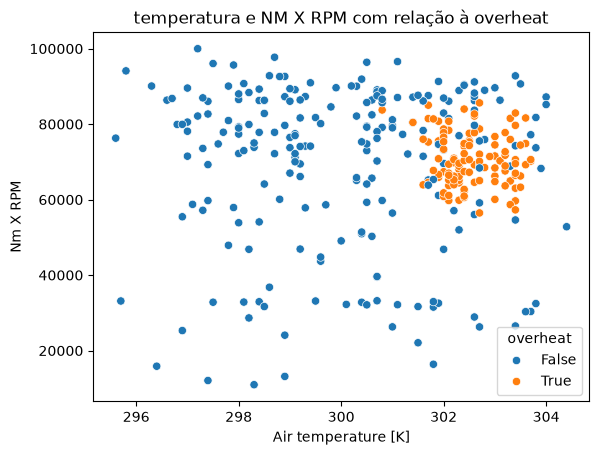
\includegraphics[width=0.8\linewidth]{overheat-relacao-temp-nmxrpm}
	\caption{\textit{Overheat} em relação a torque RPM e temperatura do ar.}
\end{figure}


\begin{figure}[h] \label{fig:torque-rpm}
	\centering
	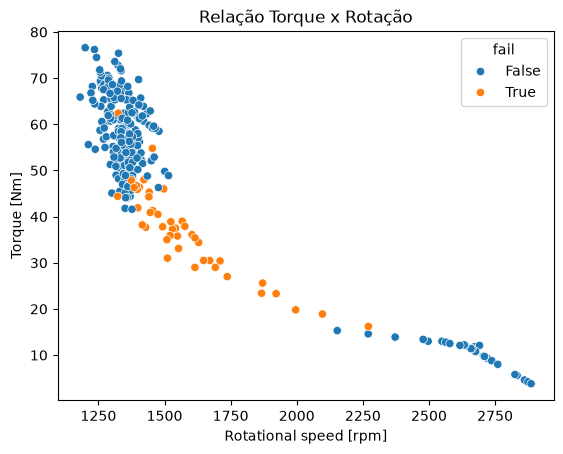
\includegraphics[width=0.8\linewidth]{rotacao-por-torque-correlacao}
	\caption{Relação de Torque por Rotação das máquinas.}
\end{figure}


\subsubsection{Tool Wear Failure}

Pra o problema de desgaste da ferramenta, foram novamente testados diferentes combinações de variáveis, como mostrado na Figura~\ref{fig:wear-vars}. Neste caso, três variáveis distintas se mostraram promissoras, sendo elas: torque, rotação e tempo de operação em minutos.

\begin{figure}[h] \label{fig:wear-vars}
	\centering
	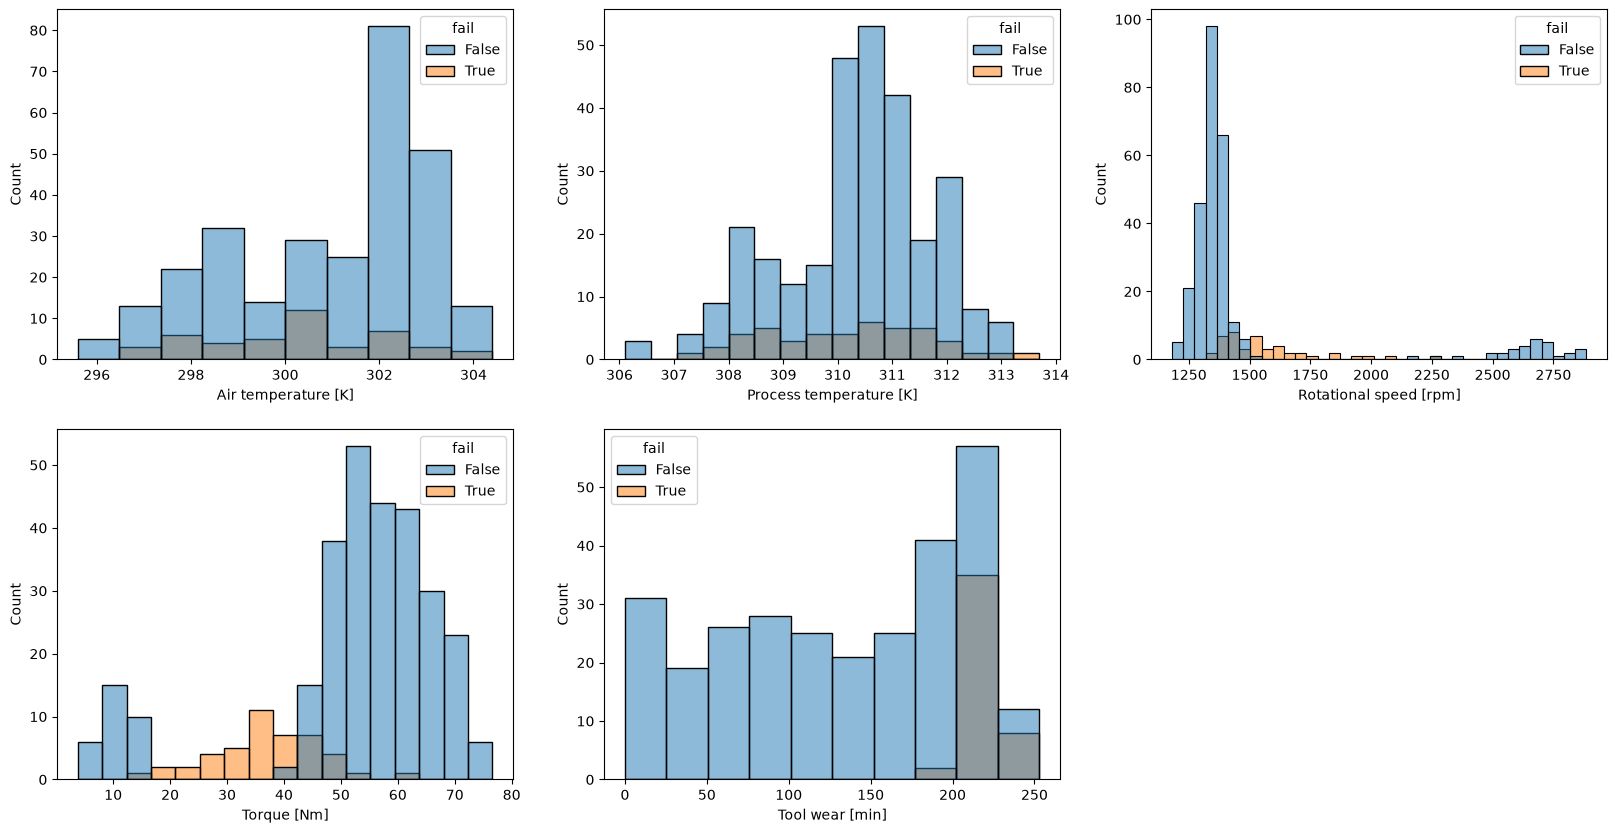
\includegraphics[width=\linewidth]{tool-wear-variaveis}
	\caption{Teste de diferentes variáveis para \textit{Tool Wear Failure}}
\end{figure}

Assim como mostrado na Figura~\ref{fig:torque-rpm}, o torque e rotação podem ser facilmente correlacionados. Assim, aplicando novamente $Nm \times RPM$, temos para falhas \textit{Tool Wear} a distribuição em Figura~\ref{fig:dist-tool-wear-rot}.

\begin{figure}[h] \label{fig:dist-tool-wear-rot}
	\centering
	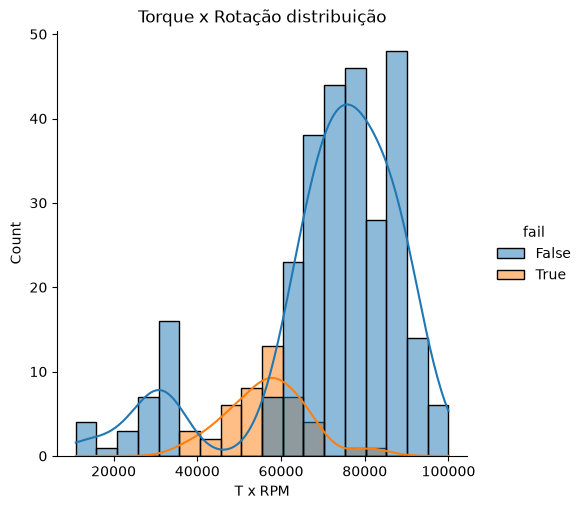
\includegraphics[width=0.8\linewidth]{dist-rotacao-por-torque}
	\caption{Distribuição de $Nm(T) \times RPM$ para falhas por desgaste.}
\end{figure}

Uma vez que Tempo de uso também estava atrelado, testou-se a possibilidade de empregar a relação anteriormente descoberta de $Nm \times Min$, entregando a distribuição em Figura~\ref{fig:dist-tool-min}. Ambas as relações mostravam distribuições centradas em um intervalo específico, o qual acreditava-se que poderia ajudar o modelo a entender rapidamente os dados.

\newpage

\begin{figure}[h] \label{fig:dist-tool-min}
	\centering
	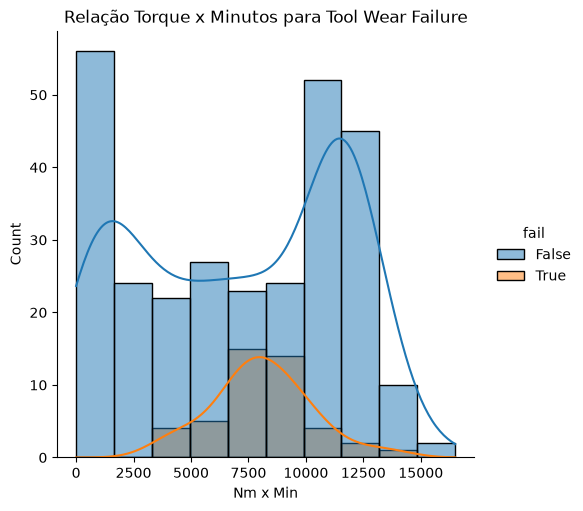
\includegraphics[width=0.8\linewidth]{toque-por-min}
	\caption{Distribuição de $Nm \times Min$ para falhas por desgaste.}
\end{figure}


\subsubsection{Power Failure}

Para problemas de energia, não tinha-se uma ideia base de o que poderia levar a classificar estes casos. Assim, uma breve exploração foi feita testando componentes, e notou-se uma distribuição evidente em relação à rotação, Figura~\ref{fig:power-rpm}.

\begin{figure}[h] \label{fig:power-rpm}
	\centering
	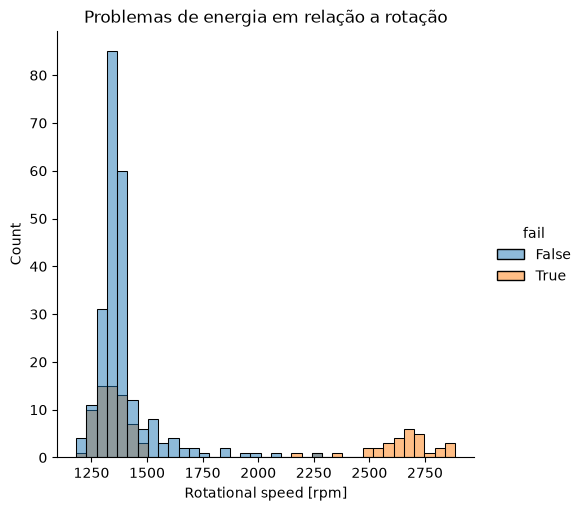
\includegraphics[width=0.8\linewidth]{energia-por-rpm}
	\caption{Rotação das máquinas em relação a falhas por energia.}
\end{figure}

Com isso, foi testado novamente a relação Torque e RPM, dado que esta já estaria presente nos dados durante o treino. Como mostrado na Figura~\ref{fig:power-nm-rpm}, a relação novamente se mostrou valida, então foi também escolhida para este caso.

\begin{figure}[h] \label{fig:power-nm-rpm}
	\centering
	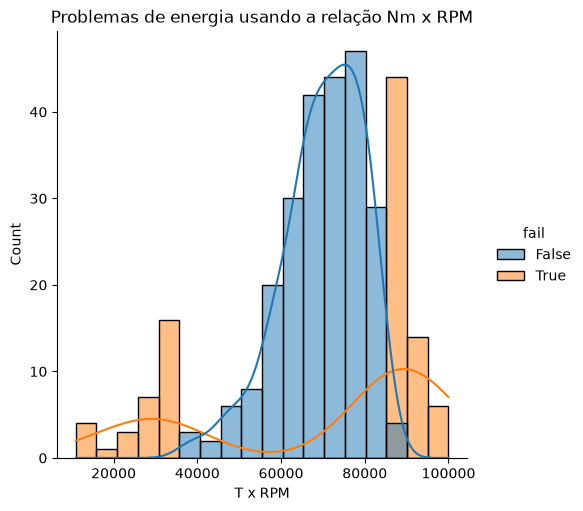
\includegraphics[width=0.8\linewidth]{energia-por-relacao-torque-por-rpm}
	\caption{Distribuição dos problemas de energia com relação a Torque e RPM.}
\end{figure}

\section{Data Augmentation e Separação dos dados}

Com as features escolhidas, sendo elas: \textbf{Nm $\times$ Min}, \textbf{Nm $\times$ RPM}, \textbf{Temperatura do Ar} e \textbf{Tipo de falha (Target)}. Foi feito um levantamento de como os dados poderiam ser usados no treinamento dos modelos.

Desde o principio, era evidente que os dados como estavam não seriam passíveis de uso, dado a gigantesca discrepância entre quantidades por classe. Assim, foi feito uma ampliação artificial dos dados.

Dado que os dados já estavam separados por falha. Adicionamos um ruído gaussiano de forma que, a soma da quantidade de dados de falhas seria aproximadamente igual a quantidade de pontos de dados sem falha. Para este trabalho, foi empregada a função \texttt{np.random.normal} do \textit{Numpy}, usando os parâmetros \texttt{mean=0; std=0.1}.

Ao final, a quantidade de dados se mostrou equivalente como mostrado na Figura~\ref{fig:igual}. Assim, ambos os dados com e sem aumento foram exportados para uso posterior.

\begin{figure}[h] \label{fig:igual}
	\centering
	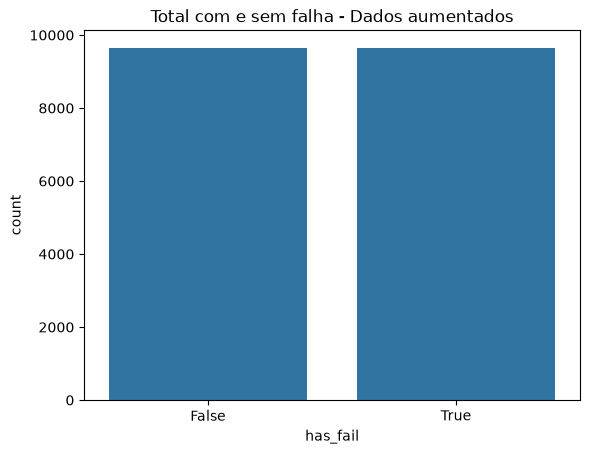
\includegraphics[width=\linewidth]{dados-augmented-total-com-e-sem-falhas}
	\caption{Equivalência de dados sem e com falhas depois do aumento artificial.}
\end{figure}

\section{Treinamento dos Modelos Default}

\bibliography{references}

\end{document}